\documentclass[12pt]{article}
\usepackage[utf8]{inputenc}
\usepackage[english]{babel}

\usepackage[a4paper, margin=1in]{geometry}

\usepackage[usenames, dvipsnames]{color}


\usepackage{graphicx}
\graphicspath{ {images/} }

\usepackage{minted}
\usepackage{mdframed}
\surroundwithmdframed{minted}

\usepackage{fancyhdr}
\pagestyle{fancy}
\fancyhf{}
\rhead{Session 1 and 2}
\lhead{Workshop: Text Analysis and Word Vectors in R}
\rfoot{Page \thepage}
\lfoot{Sara J Kerr. Frankfurt - Jan 2017}


\usepackage{hyperref}
\hypersetup{
    colorlinks=true,
    linkcolor=RoyalPurple,     
    urlcolor=OliveGreen,
}
 
\urlstyle{same}

\title{Workshop: Text Analysis and Word Vectors in R}
\author{Sara J Kerr M.A. 
 \thanks{PhD Candidate at An Foras Feasa: Maynooth University Institute for the Humanities, Ireland. \newline Supported by a Hume Scholarship.}} 
\date{January 2017}


\begin{document}
\sffamily
\setlength{\parindent}{0pt}
\setlength{\parskip}{1em}

\begin{titlepage}
\maketitle
\end{titlepage}

\tableofcontents

\section*{Overview}
This workshop will provide an introduction to textual analysis and word vector analysis in R.  R is a free and open source piece of software traditionally used for statistical analysis. Packages for R can be installed from the CRAN website via R Studio or directly from a source.

The workshop aims to introduce textual analysis and word vectors using R and provide a starting point for further exploration. The materials used will be texts in English and other European languages. Session 1 will explore some basic text analysis using R, in particular frequency analysis and Key Word in Context. While these are not necessary for using word vectors, they are helpful for putting the results of the vector space model into context and allow exploration at text level.

To apply the analysis in Workshop Session One to Japanese, the chosen texts will need to be split into words using a package like \textbf{RMeCab} (which can be found at: \textbf{\url{http://rmecab.jp/wiki/index.php?RMeCab}}) as the function used to separate the texts into word lists relies upon an regular expression and gaps between words. Unfortunately I can't give further instructions on the use of this package as the website is in Japanese. Another useful package is \textbf{Nippon} which includes a variety of utilities for handling Japanese text. 

For more advanced exploration of texts there is \textbf{Stylo} a package for stylometric analysis which has options for use with Chinese and Japanese text. For further information about the Stylo package see \textbf{\url{https://cran.r-project.org/web/packages/stylo/stylo.pdf}}, \textbf{\url{https://journal.r-project.org/archive/accepted/eder-rybicki-kestemont.pdf}}, or \textbf{\url{https://my.vanderbilt.edu/digitalhumanities/using-r-for-stylometric-analysis-with-the-stylo-package/}}.

Session 1, subsections 1--4 are adapted from Matthew L. Jockers (2014) \textit{Text Analysis with R for Students of Literature}.
Session 1, subsection 5 is adapted from blog post \textbf{\url{https://eight2late.wordpress.com/2015/05/27/a-gentle-introduction-to-text-mining-using-r/}}.
Session 2 is adapted from Benjamin Schmidt's (2015) blog post \textbf{\url{http://bookworm.benschmidt.org/posts/2015-10-25-Word-Embeddings.html}} and my doctoral research 'Jane Austen in Vector Space' presented at JADH (2016), which can be found here: \textbf{\url{https://sarajkerr.com/talks-and-papers/}}.

\section{Workshop Session One: Text Analysis in R}
You need to create a folder called Workshop on your desktop for the workshop materials and results. Folder names should not contain any gaps as this can cause problems when accessing them from R Studio. 

Open R Studio.

Before you start you need to set your `working directory', this is the folder where the texts and results are stored. Go to \textit{Session} - \textit{Set Working Directory} - \textit{Choose Directory} then browse to the folder \textit{Workshop} on your desktop.

\begin{figure}[H]
	\centering
	\includegraphics[width=0.75\textwidth]{setdir.jpg}
	\caption{Setting the Working Directory}
\end{figure}
 
 You will notice that a piece of code has appeared in the R console:

 \begin{minted}
[fontsize=\footnotesize,
linenos
]
{r}  
setwd("pathway to the working directory")

# This is the function that sets the working directory
\end{minted}
 
\subsection{Load and Preprocess a File}
This first section focuses on frequency analysis using base R. It will cover:
\begin{itemize}
\item{}
\end{itemize}

To load the first file and view the first 6 elements: 

\begin{minted}
[fontsize=\footnotesize,
linenos
]
{r} 
ja_ch <- scan("Austen_Texts/Chapter_Files/PP1_En.txt", what = "character", 
              sep = "\n")

# This can also be done using
mytext <- scan(file.choose(), what ="character", sep = "\n") 
# which allows you to search for the file you want

# A character file has been created with 80 elements.

head(ja_ch)
\end{minted}

The output will show the first 6 lines of the document - in this case the title and first 4 lines of Chapter 1 of Jane Austen's \textit{Pride and Prejudice}. Each line is enclosed in speech marks as they are character strings. You will also notice that a value \textbf{ja{\_}ch} is now in the environment pane, each time you create something it will appear in this pane. This is a character (chr) vector which has 80 elements. To access an individual element or a selection of elements:

\begin{minted}
[fontsize=\footnotesize,
linenos
]
{r} 
ja_ch[1]
ja_ch[3:4]
\end{minted}

Now create a new vector which only contains the chapter text:
\begin{minted}
[fontsize=\footnotesize,
linenos
]
{r} 
ja_ch1 <- ja_ch[3:80]
# Check the first 6 lines 
head(ja_ch1)
\end{minted}

Load the second chapter \textbf{PP1{\_}De.txt} into a vector called \textbf{ja{\_}ch{\_}d}. Create a vector which removes the first two lines and saves the chapter text into a new vector called \textbf{ja{\_}ch1d}. You should now have a character vector which contains a bad German translation of the first chapter of \textit{Pride and Prejudice} (thanks to Google Translate).  

Remove line breaks from each file (if you wish to start over in the same session rerun these two lines of code to recreate the unprocessed text). It is a good idea to keep a vector of the text in an unprocessed form, if you make a mistake you won't have to start from the beginning.

\begin{minted}
[fontsize=\footnotesize,
linenos
]
{r} 
text1 <- paste(ja_ch1, collapse = " ")
text2 <- paste(ja_ch1d, collapse = " ")
\end{minted}

The chapters are each now a single character string.

Before word frequencies can be calculated, the text needs to be processed. The level of processing will depend on the text and its language. For the texts we are using we will change the text to lower case, and extract the words saving them as a vector .

\begin{minted}
[fontsize=\footnotesize,
linenos
]
{r} 
# Change text to lower case
text1 <- tolower(text1) 
# Check in the environment pane - the capital letters have now been removed

# select words only
text1 <- strsplit(text1, "\\W") # The second argument is a regular expression

# If we look in the environment pane text1 is now a 'List of 1'
text1 <- unlist(text1) # simplify to a vector
text1
\end{minted}

Most of the chapter is now displayed (R 	has a `maximum print' limit), but where there was punctuation there are now ``'' indicating an empty space. Our next step is to remove these.

\begin{minted}
[fontsize=\footnotesize,
linenos
]
{r} 
text1 <- text1[which(text1 != "")] # '!=' means 'does not equal'
# This subsets the vector by removing elements which are not spaces
text1
\end{minted}

\textbf{text1} is now a character vector where each word is an element. If we look at the environment pane we can see the length of the vector in square brackets - 852. This gives us the number of tokens (words) in the text. It is also possible to calculate the length of a vector directly in R:

\begin{minted}
[fontsize=\footnotesize,
linenos
]
{r} 
length(text1)
\end{minted}

Now do the same for \textbf{text2}.

\subsection{Tokens, Types and Word Frequency}
This section will cover:
\begin{itemize}
\item{}
\end{itemize}

You can search for a word by its index number - R starts indexing at 1 - or by using the \textbf{which()} function. The \textbf{which()} function will return the index numbers of all occurrences of the selected word. By using the \textbf{length()} function we can identify how many times a word appears in the text. We can also use the \textbf{unique()} function to identify the word types in the text.

\begin{minted}
[fontsize=\footnotesize,
linenos
]
{r} 
text1[42]
text2[723]

which(text1 == "neighbourhood")
which(text2 == "nachbarschaft")

# number of times a word appears in the text
length(text1[which(text1 == "neighbourhood")])

# number of types in the text
length(unique(text2))
\end{minted}

Now we will use R to create a raw frequency table, sort it by most frequent words and view the top 10 as a list and as a simple plot. 

\begin{minted}
[fontsize=\footnotesize,
linenos
]
{r} 
# create a table of frequencies
text1_freqs <- table(text1)

# sort by frequency
sorted_text1 <- sort(text1_freqs, decreasing = TRUE)

# View the top 10 most frequent words in the text
sorted_text1[1:10]

# View as a plot
plot(sorted_text1[1:10])
# If all 10 words don't appear click on the Zoom option in the plot pane.
\end{minted}

Although it can be interesting to view the raw frequencies, calculating the relative frequencies allows for comparisons to be made across and between texts. The code below calculates the relative frequencies and plots the top ten words. This time we are going to add a title to the plot and custom x and y-axis titles. 

\begin{minted}
[fontsize=\footnotesize,
linenos
]
{r} 
# To calculate the relative frequencies
rel_freqs_text1 <- 100 * (sorted_text1 / sum(sorted_text1))

# Plot top 10 relative frequencies
plot(rel_freqs_text1[1:10], type = "b", main= "Relative frequencies in PP Ch 1",
        xlab = "Top Ten Words", ylab = "Percentage of Chapter")
# If all 10 words don't appear click on the Zoom option in the plot pane.
\end{minted}

\subsection{Exploring Word Frequency Across a Novel}
This section will cover:
\begin{itemize}
\item{}
\end{itemize}

So far we have focused on a single chapter - now we will briefly explore a full novel, Jane Austen's \textit{Mansfield Park}. Rather than calculating the relative frequencies for the whole novel, which we can do using the code we used for the individual chapter, we are going to calculate the relative frequencies per chapter using a regular expression.

\begin{minted}
[fontsize=\footnotesize,
linenos
]
{r} 
# Load the text into R
text_MP <- scan("Austen_Texts/Novel_Files/Austen_1814_MP.txt", 
                what = "character", sep = "\n")

# View the first 6 lines of the file
head(text_MP)

# Using regular expressions to identify chapter index positions
chapters <- grep("^CHAPTER \\d", text_MP)

text_MP[chapters]

# Add an end point to the novel and add to chapters
text_MP <- c(text_MP, "END") # the length of text_MP is increased by 1
finish <- length(text_MP)
chapters <- c(chapters, finish) 

# Calculating the word frequencies by chapter using a for loop

ch_raw_freqs <- list() # Creating empty lists to be filled by the loop
ch_rel_freqs <- list()

for(i in 1:length(chapters)) {
        if(i != length(chapters)){
                ch_title <- text_MP[chapters[i]]
                start <- chapters[i] + 1
                end <- chapters[i + 1] - 1
                ch_lines <- text_MP[start:end]
                ch_text <- tolower(paste(ch_lines, collapse = " "))
                ch_text <- strsplit(ch_text, "\\W")
                ch_text <- unlist(ch_text)
                ch_text <- ch_text[which(ch_text != "")]
                ch_freqs <- table(ch_text)
                ch_raw_freqs[[ch_title]] <- ch_freqs
                rel_ch_freqs <- 100 * (ch_freqs / sum(ch_freqs))
                ch_rel_freqs[[ch_title]] <-rel_ch_freqs
        }
}

# To find out the frequency of a word across each chapter
marriage <- lapply(ch_rel_freqs, '[', "marriage")

head(marriage) # shows the relative frequency per chapter

marriage_com <- do.call(rbind, marriage) # Combines the results by row

head(marriage_com) # This creates a matrix
\end{minted}

The matrix created in R now appears in the environment pane under \textbf{data}. There is a small spreadsheet icon on the right hand side of the entry, if you click this the matrix will open in the document editor pane.

However, it is easier to view the different frequencies of words by plotting them next to each other. In this next example we will compare the relative frequency of `he' and `she' in the novel by plotting them next to each other:

\begin{minted}
[fontsize=\footnotesize,
linenos
]
{r} 
# Compare instances of 'he' and 'she' in the novel
he <- lapply(ch_rel_freqs, '[', "he")
he_com <- do.call(rbind, he)
she <- lapply(ch_rel_freqs, '[', "she")
she_com <- do.call(rbind, she)

# Extract the relative frequencies and combine in columns
he_rf <- he_com[, 1] 
she_rf <- she_com[, 1] 
# This extracts all rows of the 1st column - to extract data from a matrix
# you use nameofmatrix[rows, columns]
# Combine the frequencies into two columns
rf_he_she <- cbind(he_rf, she_rf)

head(rf_he_she)

# Create a plot comparing the frequencies side by side
barplot(rf_he_she, beside = TRUE, col = "red")
\end{minted}

Once you have created a relative frequencies list you may wish to compare a variety of different words. Rather than rewriting the code each time we can create a function that allows us to do the comparison with a single line of code.

\begin{minted}
[fontsize=\footnotesize,
linenos
]
{r} 
# The arguments for the function are the chapter relative frequencies and 
# your two chosen words - the words need to be in speech marks
rel_freq_comp <- function(ch_rel_freqs, word1, word2) {
        worda <- lapply(ch_rel_freqs, '[', word1)
        worda_com <- do.call(rbind, worda)
        wordb <- lapply(ch_rel_freqs, '[', word2)
        wordb_com <- do.call(rbind, wordb)
        worda_rf <- worda_com[, 1] 
        wordb_rf <- wordb_com[, 1] 
        rf_a_b <- cbind(worda_rf, wordb_rf)
        # This changes the column names to your chosen words
        colnames(rf_a_b) <- c(word1, word2) 
        barplot(rf_a_b, beside = TRUE, col = "red", 
                main = "Relative Frequencies By Chapter")
}

# To use the function to compare the names of the two main characters
rel_freq_comp(ch_rel_freqs, "fanny", "edmund")
\end{minted}

\subsection{Handling Multiple Files and Key Word in Context}
This section will cover:
\begin{itemize}
\item{}
\end{itemize}

If we want to look at a corpus of texts we need to have a way of identifying the files we wish to examine. To do this, we will create functions to list the files in a folder and to create a word list from each of the files. The time this takes will depend upon the number of files in the folder and their size.

\begin{minted}
[fontsize=\footnotesize,
linenos
]
{r} 
# Create a path to the files
input.dir <- "Austen_Texts/Novel_Files" 
# Read the name of all .txt files
files <- dir(input.dir, "\\.txt") 

# Create a function to list the files
show_files <- function(files){
        for(i in 1:length(files)){
                cat(i, files[i], "\n", sep = " ")
        }
}

# To use the function:
show_files(files) # the files are listed and numbered

# Create a function to create a list of words from each file, you will recognise
# the code from the previous sections

make_word_list <- function(files, input.dir) {
       # create an empty list for the results
        word_list <- list()
        # read in the files and process them
        for(i in 1:length(files)) {
             text <- scan(paste(input.dir, files[i], sep = "/"), 
                          what = "character", sep = "\n")   
             text <- paste(text, collapse = " ")
             text_lower <- tolower(text)
             text_words <- strsplit(text_lower, "\\W")
             text_words <- unlist(text_words)
             text_words <- text_words[which(text_words != "")]
             word_list[[files[i]]] <- text_words
        }
        return(word_list)
}

# To use the function:
my_corpus <- make_word_list(files, input.dir) 
\end{minted}

If you scroll down to the bottom of the environment pane you will see the heading \textbf{functions} and the three functions we have created will be listed.

To explore individual words within the context they appear in, we can use Key Word in Context. We will create a \textbf{kwic} function which uses the output from the \textbf{make{\_}word{\_}list()} function and uses the \textbf{show{\_}files()} function. This means that before you run the \textbf{kwic()} function you will need to check that \textbf{make{\_}word{\_}list()} and \textbf{show{\_}files()} functions are listed.

\begin{minted}
[fontsize=\footnotesize,
linenos
]
{r} 
# Creating a Key Word in Context (KWIC) function - this uses the output from
# the make_word_list and includes the show_files function 

kwic <- function(my_corpus) {
        show_files(names(my_corpus))
        # identify the chosen file
        file_id <- as.numeric(
          readline("Which file would you like to examine? Enter a number: \n"))
        # identifythe number of words each side of the keyword
        context <- as.numeric(
                readline("How much context do you want? Enter a number: \n"))
        # identify the focus word
        keyword <- tolower((readline("Enter a keyword: \n")))
        # create the KWIC readout
        hits <- which(my_corpus[[file_id]] == keyword)
        if(length(hits) > 0) {
                result <- NULL
                for(j in 1:length(hits)) {
                        start <- hits[j] - context
                        if(start < 1) {
                                start <- 1
                        }
                        end <- hits[j] + context
                        cat("\n--------------------", j, "----------------\n")
                        cat(my_corpus[[file_id]][start:(hits[j] -1)], sep = " ")
                        cat("[", my_corpus[[file_id]][hits[j]], "] ", sep = " ")
                        cat(my_corpus[[file_id]][(hits[j] +1): end], sep = " ")
                        myrow <- cbind(hits[j],
                                paste(my_corpus[[file_id]][start: (hits[j] -1)],
                                      collapse = " "),
                                paste(my_corpus[[file_id]][hits[j]],
                                      collapse = " "),
                                paste(my_corpus[[file_id]][(hits[j] +1): end],
                                      collapse = " "))
                        result <- rbind(result, myrow)
                }
                colnames(result) <- c("position", "left", "keyword", "right")
                return(result)
        } else {
                cat("YOUR KEYWORD WAS NOT FOUND\n")
        }
}

# To use the function:
results <- kwic(my_corpus)
# select the file, context and keyword when prompted

# If you wish to save the results as a .csv file
write.csv(results, "Results/yourkeyword_text.csv")
# e.g. if the chosen word was marriage in Mansfield Park
write.csv(results, "Results/marriage_MP.csv")
\end{minted}

\subsection{Using the 'tm' Package}
This section will cover:
\begin{itemize}
\item{}
\end{itemize}

An alternative to working in base R is to use the `tm' text mining package. The package is designed specifically for text mining a corpus and offers a variety of tools. An introduction to the `tm' package can be found here: \textbf{\url{ftp://cran.r-project.org/pub/R/web/packages/tm/vignettes/tm.pdf}}. 

Begin by clearing your workspace, this can be done by clicking on the broom in the environment pane or choosing \textit{Session} - \textir{Clear Workspace}. This will remove all the objects created during the previous session.

We start by telling R where the files we are using are stored, in this case the Novel_Files folder.

\begin{minted}
[fontsize=\footnotesize,
linenos
]
{r} 
# Tell the computer where the texts are located
dname <- file.path("Austen_Texts/Novel_Files") # Tells R the path to the files
dname
dir(dname) # Lists the files in the directory/folder
\end{minted}

As we are using a number of packages for this session which do not come as part of base R they need to be installed and loaded for use. There are two ways to add packages to R in R Studio, the first is by using the \textit{Tools - Install Packages} option in the top menu in R Studio.

\begin{figure}[H]
	\centering
	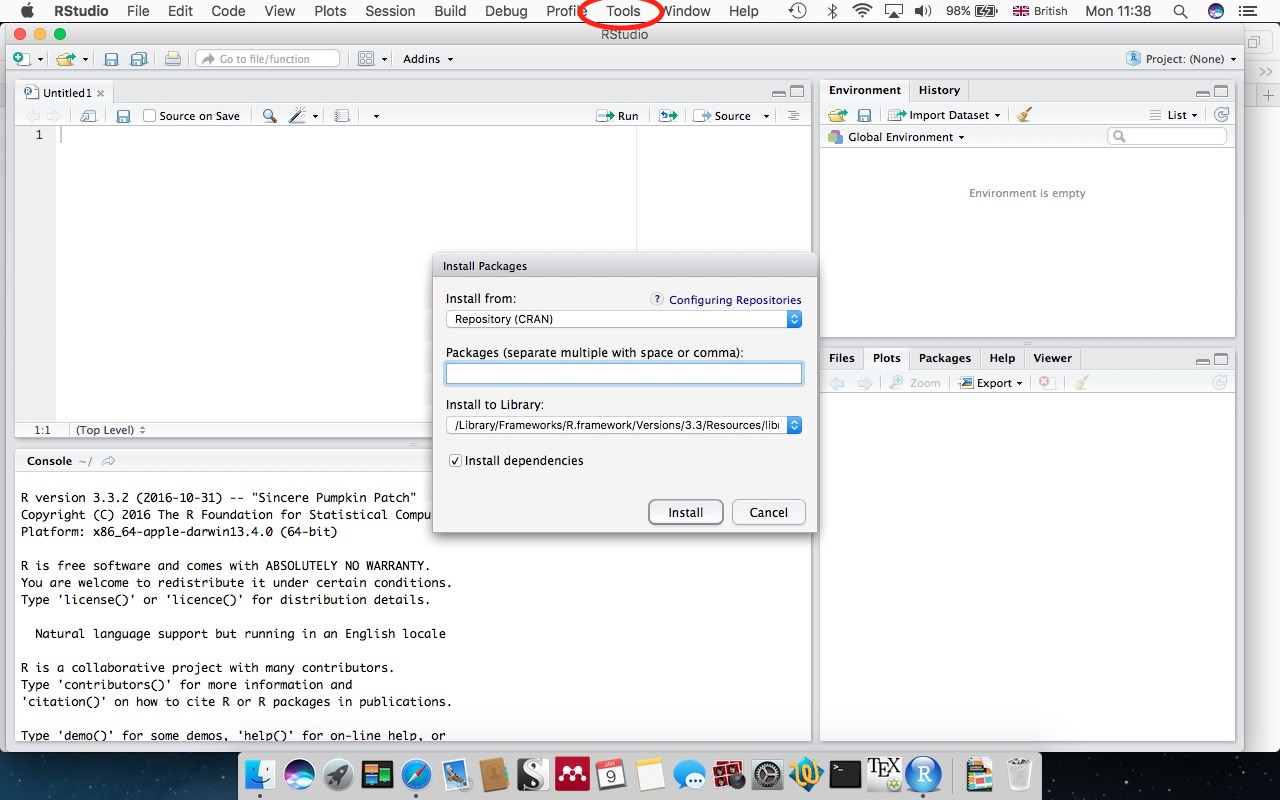
\includegraphics[width=0.75\textwidth]{installPkg.jpg}
	\caption{R Studio Install Packages}
\end{figure}

You will need to write the name of each package you wish to download separated by a comma or space. However, this will only work for packages which are available from the CRAN website. Alternatively, packages can be downloaded from the command line:

\begin{minted}
[fontsize=\footnotesize,
linenos
]
{r} 
install.packages("name of packages")
\end{minted}

It may take a little time for all the packages to install. Once this has been done, and the command prompt \textbf{\textgreater} is showing, you can continue. To load the packages you need to tell R you want to use them. We are going to use \textit{tm}, \textit{ggplot2} and \textit{wordcloud}.

\begin{minted}
[fontsize=\footnotesize,
linenos
]
{r} 
library(tm) # tm is a text mining package
library(ggplot2) # ggplot2 is a graph plotting package
library(wordcloud) # lets you create wordclouds
\end{minted}

Now we have loaded the packages we want to use we need to load the corpus into R using the \textbf{tm} package. This will create a V or volatile corpus which means that it only exists in the current session of R. Next we will process the corpus removing punctuation, numbers, uppercase letters and white spaces. We could also remove stopwords, but we won't do that at the moment.

\begin{minted}
[fontsize=\footnotesize,
linenos
]
{r} 
# load the corpus
docs <- Corpus(DirSource(dname)) 

# Preprocess the text
docs <- tm_map(docs, removePunctuation)   # Remove punctuation   
docs <- tm_map(docs, removeNumbers)      # Remove numbers    
docs <- tm_map(docs, tolower)   # Convert to lowercase   
# docs <- tm_map(docs, removeWords, stopwords("english")) # To remove stopwords 
docs <- tm_map(docs, stripWhitespace)   # Strip whitespace   
docs <- tm_map(docs, PlainTextDocument) 
# This is the end of the preprocessing stage.
\end{minted}

Once the corpus has been processed a Document Term Matrix (DTM) can be created. The DTM is a matrix which describes the frequency of terms in the corpus where each row is a document and each column is a word or term from the corpus.

\begin{minted}
[fontsize=\footnotesize,
linenos
]
{r} 
# Create a Document Term Matrix
dtm <- DocumentTermMatrix(docs)   

# To view or export the DTM
corpus_dtm <- as.matrix(dtm)
rownames(corpus_dtm) <- c("PP", "MP")

# It is also possible to create a Term Document Matrix
tdm <- TermDocumentMatrix(docs)
corpus_tdm <- as.matrix(tdm)
colnames(corpus_tdm) <- c("PP", "MP")

# Write files to a folder
write.csv(corpus_dtm, "Results/dtm.csv")
write.csv(corpus_tdm, "Results/tdm.csv")

# Explore your data - this gives the raw frequency for each word in the corpus      
freq <- colSums(as.matrix(dtm))   
length(freq)   # the number of unique words in the corpus
head(freq) # view the top 6 elements
\end{minted}

It can be useful to visualise the word frequencies. Below are two examples, a frequency graph showing words which appear more than 500 times, and word clouds showing 100 words and words with a minimum frequency of 100.

\begin{minted}
[fontsize=\footnotesize,
linenos
]
{r} 
# Create a frequency graph of the words which appear more than 500 times  
  
word_freq <- data.frame(word=names(freq), freq=freq)   
p <- ggplot(subset(word_freq, freq>500), aes(word, freq))    
p <- p + geom_bar(stat="identity")   
p <- p + theme(axis.text.x=element_text(angle=45, hjust=1))   
p  

# Create a wordcloud
  
set.seed(142)   # set.seed is used to ensure replicability
wordcloud(names(freq), freq, max.words=100)   

set.seed(142)   
wordcloud(names(freq), freq, min.freq=100, scale=c(5, .1), 
          colors=brewer.pal(8, "Set1"))  # This section determines the colours
\end{minted}

You could rerun the code applying the stopword option to see the difference it makes to the visualisations.
 
\begin{minted}
[fontsize=\footnotesize,
linenos
]
{r} 

\end{minted}
\newpage
\section{Workshop Session Two: Work Vectors in R}
This section will cover:
\begin{itemize}
\item{}
\end{itemize}
Hello, here is some text without a meaning.  This text should show what 
a printed text will look like at this place.




\end{document}